\section{Equilibrium analysis}
In this chapter, we study the equilibrium outcomes of the theoretical model using numerical simulations. We first describe how our algorithm works and how we choose the values of the main parameters. Then, we present the results of the simulations under different parameter configurations and study how the equilibrium outcomes change. We find that the agents choose the RN option in all equilibria, but in the first they exert high effort and pick high volatility, whereas in the second and third bests they exert low effort but still pick high volatility. These results are robust to changes in most parameters, but quite sensible to the optimal stopping time and to the difference between the two effort levels. Finally, we consider briefly special cases of the model, namely when the executive can choose only effort, only volatility, or only the RN option, and find that leaving the executive the possibility to choose (high) volatility is Pareto improving.


\subsection{Parameter Choice and Algorithm Design}
We first discuss the choice of parameters for the simulations. A complete list can be found in the Online Appendix,
therefore we will just focus on the ones that need to be shortly discussed. We set the risk-free rate $r$ to 0.045, which is the current rate of the 10-Year US Treasury Rate as of May 14th, 2021 \citep{ychartrfrate}, and the volatility $\bar{\sigma}$ to 0.3, as is done in the (older) literature, which is not far away from the volatility observed in the past few years. For our Brownian motion, we choose a time horizon of 20 years, which is the maximum time a reload option can be out before being fully exercised. We then run $100$ paths and $5,000$ points, which is approximately one point per trading day over 20 years, and is sufficient for our purposes. For simplicity, we assume the stock has zero drift. The most delicate choice involves the average number of years until the RN option is exercised $y_{RN}$, as well as the R option's first and second exercise, respectively $y_{R1}$ and $y_{R2}$. We choose $y_{RN} = 7$ based on the available empirical literature (Table 4 in \citet{murphy2019employees}), $y_{R2} = 7$ since the remaining part is a RN option, and assume $y_{R1}$ to be slightly lower and set it thus to 6. These choices are key since they influence both the stock price evolution --- they determine when effort and additional volatility cease --- and the agent's utility, as her wealth depends on whether and how many times the option has been exercised. As we will see, robustness checks show indeed that these parameters are relevant and influence the final results. For computational reasons, we set $N\_init = 500$ and $N\_init\_r = 50$; our tests show that the latter provides nevertheless a good approximation of the cost of the R option, as we still have a total of 500 steps over the lifetime of the option. We set the number of agents to 10, which seems a reasonable number for a C-suite. Agents have a 67-33 portfolio, meaning that 67\% of their outside wealth is invested into firm stock and the remaining 33\% in cash; we set the exact numbers by replicating \citet{carpenter1998exercise}. We also test the case with the executive holding a 50-50 portfolio, but results do not change significantly. For the $R_{\alpha, \gamma}$ option, we allow $\alpha$ to take value in $A = \{0.2, 0.5, 0.6, 0.7, 0.75, 0.8, 0.9, 1\}$ and $\gamma$ in $\Gamma = \{0, 0.05, 0.1, 0.15, 0.2, 0.25, 0.5, 0.75, 1\}$; ideally we would like $\alpha$ and $\gamma$ to take values in the continuum $[0, 1]$, but we are forced to choose these discrete subsets for computational reasons. Finally, the remaining relevant choices are the high and low values of the coefficient of risk aversion $\rho$, the effort $a$, and the volatility $\sigma$. We set $\rho_L = 1.5$ and $\rho_H = 2.5$, $a_L = 0$ and $a_H = 1$, and $\sigma_L = 0$ and $\sigma_H = 0.01$. The values of $\rho$ are taken from \citet{carpenter1998exercise}, while the latter are fine-tuned for realistic behavior of the stock price and utility functions. 

\subsubsection*{Algorithm}
We now provide a brief overview of the algorithm that returns the equilibrium outcomes. First, we simulate the stock price path by constructing an array of possible paths over the given timeframe, considering the relevant effort and volatility levels that influence the stock price, up until when the option is not fully exercised, reload option included. We discretize the stock's Geometric Brownian motion using the Python implementation of \citet{qsbrownianpy}, which is based on the theoretical framework of \citet{glasserman2004monte}. 
\vspace*{15pt}
\begin{figure}[H]
    \centering
    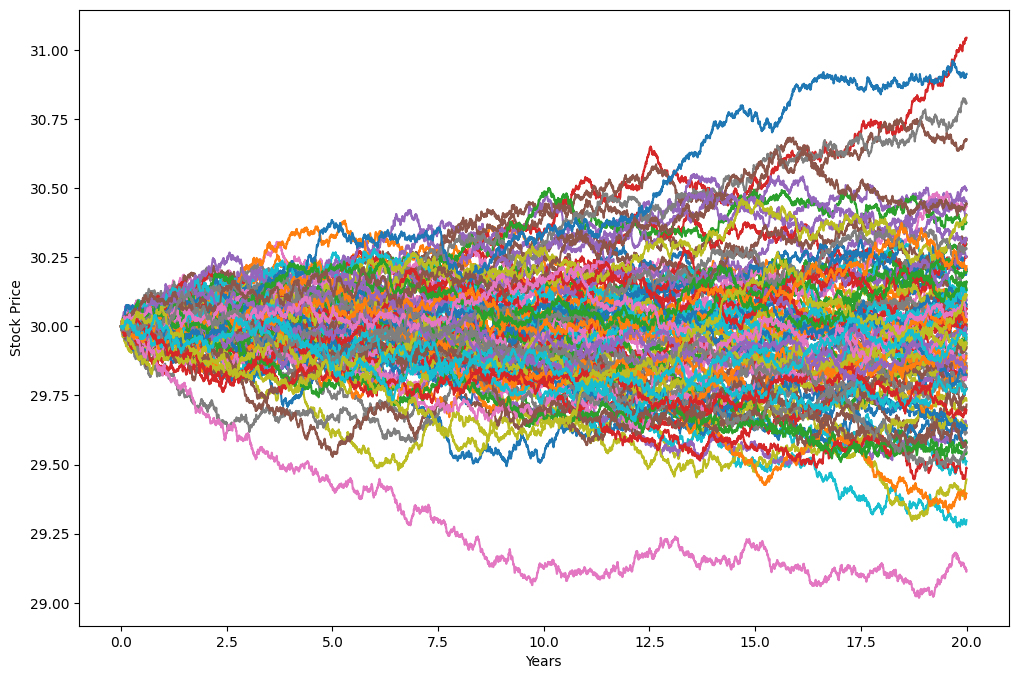
\includegraphics[width=0.6\textwidth]{fig/5/sim_motion.png}
    \caption{Simulation of possible price paths for a stock with zero constant mean, zero additional mean, zero additional volatility}
    \label{fig:sim_motion}
\end{figure}
\vspace*{15pt}

We then compute the agent's utility using the risk-free rate $r$ for discounting, with the expectation being taken over all possible Brownian motion paths computed before. The agent's wealth at time $t$ depends on whether and how many times the option has been exercised. On the other hand, the expected value of the terminal stock price is simply $E[S_T] = S_0 * e^{a_{tot}*t}$, where $a_{tot}$ is the sum of the efforts of all executives. Note that volatility does not play a role in the expectation, which reflects the risk neutrality of the principal. Therefore, the choice of volatility is relevant as long as it gives some benefit to the agent (i.e., it increases her utility), or if the principal really wanted to implement a specific project with a given volatility, known to him.
From here, the principal proposes some R option, i.e., chooses $\alpha$ and $\gamma$, and the agent chooses the controls $a^* \in \{a_L, a_H\}$, $\sigma^* \in \{\sigma_L, \sigma_H\}$, and the option $\theta^* \in \{ \theta_R, \theta_{RN} \}$, which are then used to simulate the stock price and compute the agent's and the principal's utilities. The principal then ranks all $(\alpha, \gamma, a^*_{\rho_L}, a^*_{\rho_H}, \sigma^*_{\rho_L}, \sigma^*_{\rho_H}, \theta^*_{\rho_L}, \theta^*_{\rho_H})$ sets based on his utility; for the first, second, and third equilibria, he checks whether the constraints are satisfied and thus gets an updated (and constrained) ordering. Clearly, if an allocation is part of some higher equilibria, it is also part of an equilibrium in all lower cases. For example, if an allocation is part of a third best equilibrium, then it must be also a first and second equilibria. Finally, the algorithm returns the ranked equilibrium allocations and outcomes, for each type of equilibrium. We label equilibria as either pooling, screening, shutdown, or no equilibrium. The first two are proper equilibria, in the sense that all the required constraints are satisfied, with the difference being if both agents have the same controls or not, while the shutdown is not, since one agent is not active and chooses the outside option. No equilibrium means that for both agents the constraints are not satisfied, which implies a cascade effect on the higher equilibria: for example, if an allocation does not satisfy the IR constraints, then it clearly cannot be neither a second nor a third best.


\subsection{Results} 
We run the base case with the parameters described before and in the Online Appendix.
\vspace*{10pt}

\begin{table}[H]
    \centering
    \resizebox{\textwidth}{!}{%
    \begin{tabular}{|cc|cccc|cccc|c|c|}

        \hline
        \multirow{2}{*}{$\alpha^*$} & \multirow{2}{*}{$\gamma^*$} & \multicolumn{4}{c}{$\rho_L$} & \multicolumn{4}{c}{$\rho_H$} & \multirow{2}{*}{$\EX[S_T]$} & \multirow{2}{*}{$\Pi$}\\
        & & $\theta^*$ & $a^*$ & $\sigma^*$ & $U$ & $\theta^*$ & $a^*$ & $\sigma^*$ & $U$ & & \\
        \hline
        A & $\Gamma$ & RN & 1 & 0/0.01 & 222.42 & RN & 1 & 0/0.01 & 24.73 & 222 & 209.39 \\
        \hline
    
    \end{tabular}%
    }

    \caption{First Best of Base Case}
    \label{tab:base_1st}
\end{table}

\vspace*{10pt}

Given our initial sets, we have a total of $4,608$ possible allocations; all of them are found to be IR-compatible as the zero reservation utility is never binding. Out of these, 288 are first best equilibria, i.e., they give the (same and) highest utility to the principal. Indeed, in the first best, the principal is best off by having both types of executives exerting high effort, and is indifferent whether they choose high or low volatility (recall that volatility does not enter directly the principal's utility). Since all agents choose the RN option --- less expensive for the principal, and convenient if it nevertheless were to induce high effort --- the choice of $R_{\alpha, \gamma}$ is immaterial and hence we have 288 possible allocations that give the principal the highest utility. But, as we will see shortly, none of them is incentive compatible for either executive. After these 288 equilibria, the following ones are ranked by decreasing cost of $R_{\alpha, \gamma}$ for the executive, and where at least one agent does not choose the RN option --- if not both, if the difference in total cost is lower than having only one agent choose the R for the next values of ($\alpha, \gamma$). Therefore, we find first the outcomes with higher $\alpha$ and lower $\gamma$, then the others.

\vspace*{10pt}

\begin{table}[H]
    \centering
    \resizebox{\textwidth}{!}{%
    \begin{tabular}{|cc|cccc|cccc|c|c|}
        \hline
        \multirow{2}{*}{$\alpha^*$} & \multirow{2}{*}{$\gamma^*$} & \multicolumn{4}{c|}{$\rho_L$} & \multicolumn{4}{c|}{$\rho_H$} & \multirow{2}{*}{$\EX[S_T]$} & \multirow{2}{*}{$\Pi$}\\
        & & $\theta^*$ & $a^*$ & $\sigma^*$ & $U$ & $\theta^*$ & $a^*$ & $\sigma^*$ & $U$ & & \\
        \hline
        A & $\Gamma$ & RN & 0 & 0.01 & 296.61 & RN & 0 & 0.01 & 98.91 & 30 & 17.71 \\
        \hline
    \end{tabular}%
    }

    \caption{Second Best of Base Case}
    \label{tab:base_2nd}
\end{table}

\vspace*{10pt}

The second and third bests are more interesting. We have $288$ allocations that are IC-compatible, but only the first $72$ are second bests, whereby the agents choose low effort, high volatility, and RN option in all of them. However, none of them was a first best and most of them are also not third bests. After these $72$ equilibria, in the remaining ones either one or both agents choose the R option, but again with low effort and high volatility. Therefore, we note that the principal is not able to induce high effort from the agent anymore. Finally, in the third best we are left with only 82 outcomes: the principal is indifferent among the first 5, which we show in Table \ref*{tab:base_3rd}. Therefore, in the third best, we have an equilibrium whereby both agents choose the RN option, exert low effort and choose the project with higher volatility. The principal chooses any between $R_{0.75, 0}, R_{0.8, 0}, R_{0.9, 0}, R_{1, 0}$, and $R_{1, 0.05}$, since in equilibrium the agent will nevertheless choose the RN option, and these are the only cases for which IC constraints are satisfied.

\vspace*{15pt}

\begin{table}[H]
    \centering
    \resizebox{\textwidth}{!}{%
    \begin{tabular}{|cc|cccc|cccc|c|c|}
        \hline
        \multirow{2}{*}{$\alpha^*$} & \multirow{2}{*}{$\gamma^*$} & \multicolumn{4}{c|}{$\rho_L$} & \multicolumn{4}{c|}{$\rho_H$} & \multirow{2}{*}{$\EX[S_T]$} & \multirow{2}{*}{$\Pi$}\\
        & & $\theta^*$ & $a^*$ & $\sigma^*$ & $U$ & $\theta^*$ & $a^*$ & $\sigma^*$ & $U$ & & \\
        \hline
        {0.75, 0.8, 0.9, 1} & 0 & RN & 0 & 0.01 & 296.61 & RN & 0 & 0.01 & 98.91 & 30 & 17.71 \\
        1 & 0.05 & RN & 0 & 0.01 & 296.61 & RN & 0 & 0.01 & 98.91 & 30 & 17.71 \\
        \hline
    \end{tabular}%
    }

    \caption{Third Best Equilibria of Base Case}
    \label{tab:base_3rd}
\end{table}
\newpage

Few comments are in order. First, we note that most equilibria are pooling: in the first best case, they are all pooling in effort whereas half is pooling and half is screening in volatility; in the second and third best instead, they are pure pooling in both effort and volatility, as agents choose low effort and high volatility. Second, as we would expect, agents' utilities increase as we move to second and third best, whereas principal's goes down. The utility of the low risk-averse executive rises from $222.42$ to $296.61$, and of the high risk-averse executive from $24.73$ to $98.91$. As such, the high risk-averse type seems to be comparatively better off. On the other hand, the principal's utility falls down from $209.39$ to $17.71$, a fall which is mostly driven by the decrease in terminal stock price, as a result of having first all, and then none agents exerting high effort, which would influence the drift of the stock price evolution.

We now test if these results are robust to changes in the key parameters, focusing first on the firm-side parameters --- number of agents, lambda, beta --- and then on the agent-side parameters --- rho, effort, sigma, years, delta, alpha.
Changing the number of agents has little effect on the second and third best allocations, since agents do not exert effort and so all utilities remain the same. The only difference is in the first best, where the principal's utility increases as the number of agents increases, since there are more executives that exert high effort and hence the stock price is higher. However, this is due to how we modeled the stock price evolution: if we were instead to consider a proportional system of total effort --- similar to how the cost of the two options is accounted for in the principal's utility --- then his utility would remain the same even as the number of agents changes. Similarly, the main findings remain the same as we change the proportion of low risk-averse agents $\lambda$: the only difference is at the extremes $\lambda = 0$ or $\lambda = 1$, where the choices of effort, volatility, and option of the non-participating agent are irrelevant, which thus artificially extends the possible allocations in the different equilibria. Indeed, what matters here is that the participating agent chooses the RN option, high volatility, and high effort in the first best and low effort in the other two equilibria; therefore, the other agent can also choose the R option in the second and third best, in principle. The results are also robust for changes in $\beta$: the main difference is that the principal is less interested in the stock price as $\beta$ decreases, and hence the equilibria are more likely to feature the RN option. Indeed, at $\beta = 0$, the principal is completely uninterested in the stock price and hence all allocations where both agents choose the RN option are first bests. This remains true also for the second and third bests, where the equilibria are pinned down by agents' incentive compatibility constraints.

Focusing on agent-side parameters, we first test against changes in the risk aversion coefficients. By changing to $\rho_H = 2$, we find the same outcomes as above but clearly a slightly higher utility for the high risk averse agent. Further changes to the risk aversion of the high type are either not very interesting, or difficult to compute because of precision issues of our code (since utility becomes very small for $\rho > 3$). The interesting case is when we increase the risk aversion of the low type, as this determines how many second bests are also third bests. For example, for $\rho_L=2$, the set of third best equilibria now includes also $R_{0.7,0}$ and $R_{0.9,0.5}$ --- but the agents still choose the RN option: the intuition is that it is now incentive compatible also for the low risk-averse agent to choose the (safer) RN option, as she is too risk-averse to choose the R option. By further increasing to $\rho_L=2.5$, the set of third best equilibria increases to 72. Therefore, the risk aversion of the low type determines how many second bests are also third bests. As mentioned before, too high risk aversion coefficients cannot be handled with our code because the difference in utilities becomes too low.
Changing $a_H$ and $a_L$ has a different behavior: increasing $a_H$ while keeping $a_L=0$ does not change the main results, whereas increasing to $a_L=0.5$ leads to a unique equilibrium with $R_{1,0}$, i.e., the RN option, which holds true even when we further increase $a_H$. We tried to make $a_L$ and $a_H$ as close as possible so to see if some agents will choose $a_H$ in a third best, but the two values seem to still be quite apart with our precision constraints. On the other hand, changing $\sigma$ has no direct effect on the principal's utility, as he is risk-neutral and is only interested in the expectation of stock price, whereas the agent still prefers high or low volatility in the first best, and high in the second and third. But they do so still with the RN option, rather than with the larger volatility exposure of the R option. Increasing volatility has decreasing returns to the agent's utility as the agent is more risk-averse, but with our sensitivities --- up to $\sigma = 0.1$, i.e., a third of stock's total volatility --- both agents still prefer high volatility. It is likely that with even higher volatility, or more realistically with more risk-averse agents, this would not hold true anymore after a certain point. Changing $\delta$ or $\alpha$ in the Brownian motion proves to be irrelevant with our base results, if not for the extreme cases: at $\delta = 0$, executive's choice of volatility is irrelevant and hence she chooses either high or low in all equilibria, while for $\alpha = 0$, the principal is only interested in the cost of the option and hence the agent chooses the RN option in all equilibria, which is the cheapest for the principal. Finally, changing the average years of exercise has an important impact on the results: as $y_{R1}$ becomes larger than $y_{RN}$, both agents would choose the $R$ option in the third best, but since effort is still 0, the principal minimizes cost and so the RN option is the only third best equilibrium. Clearly, the low risk-averse type is the first to prefer the R option in the other cases, i.e., she has the first to have the second set of incentive compatibility constraints satisfied. This suggests that the choice of this parameter requires great care, as it can change the equilibrium outcomes significantly, and so should be investigated further via empirical evidence, if not modeled drawing from optimal stopping theory. 

We test some special cases and find that the results are not quite surprising. By setting $A=\{1\}$, $\Gamma=\{0\}$ we are \textit{de facto} only allowing for the RN option, which does not change our main results but leads only to a unique equilibrium allocation in the third best, since the other 4 allocations with the R option are not available anymore. If we allow the executives to choose only the volatility, only the principal is worse off in the first best because he does not enjoy the stock price appreciation due to higher effort. On the other hand, if they can choose only the effort,  in the third best the principal is indifferent whereas the agent is worse off, as she would prefer to choose some additional volatility. Therefore, it seems Pareto improving to allow executives to control part of firm's volatility, as this increases their utility while leaving the (risk-neutral) firm indifferent. 

Finally, we re-run everything with a 50-50 agent, and find that the results and sensitivities do not change significantly.